%Vor dem Editieren die Styleguide auf dem Server lesen!
%Include Header
%Angaben zum Dokument
\newcommand*\myauthor{Gian Claudio K�ppel}
\newcommand*\mytitle{Elektrotechnik 2 Zusammenfassung}
\newcommand*\mydate{21.02.2011}

%Schriftgroesse, Layout, Papierformat, Gleichungen Linksbuendig
\documentclass[10pt,twoside,a4paper,fleqn]{article}

%Abmessungen Layout
\usepackage[left=1cm,right=1cm,top=1cm,bottom=1cm,includeheadfoot]{geometry}

%Package fuer Umlaute
\usepackage[latin1]{inputenc}
\usepackage[T1]{fontenc}
\usepackage[latin1]{inputenc}

%Package fuer Deutsch
\usepackage[ngerman]{babel}

%Formeln
\usepackage{amsmath}
%Spezielle Symbole in Formeln
\usepackage{amssymb}
%Sonderzeichen
\usepackage{textcomp}
%Bilder und Grafiken
\usepackage{graphicx}
%Textfarben
\usepackage{color}
%Fliesstext
\usepackage{wrapfig}
%Header und Footer
\usepackage{fancyhdr}
%Teile des Dokuments Mehrspaltig
\usepackage{multicol}
%Mehere Zellen vertikal verbinden
\usepackage{multirow} 
%Rotieren von Elementen (Bilder, Tabellen...)
\usepackage{rotating}
%Schriftart
\usepackage[scaled]{helvet}
\renewcommand*\familydefault{\sfdefault}
%Multirow
\usepackage{multirow}

%Seitenaufbau
\pagestyle{fancy} %eigener Seitenstil
%\fancyhf{}

%Linker Header
\lhead{\mytitle}


%Rechter Header
\rhead{\leftmark}
%Linker Footer
\lfoot{\myauthor}
%Center Footer
\cfoot{\thepage}
%Rechter Footer
\rfoot{\mydate}
%Text Linksbuendig, unregelmaessiger rechter Rand
\raggedright


%Document Anfang
\begin{document}

%Input von Kapiteln anschliessend
%\input{sections/kapitelname}
%Input von Kapiteln auf neuer Seite
%\include{sections/kapitelname}
%%Kreiert eine nervige erste Seite damit das dumme Fussvolk endlich lernt dass es
% nicht einfach ist eine Zusammenfassung zu schreiben. Hoffentlich bekommen wir
% dadurch mehr Nazigold!

%Damit die Seite eingebunden wird folgende Zeile ohne % ins mainfile kopieren:
%%Kreiert eine nervige erste Seite damit das dumme Fussvolk endlich lernt dass es
% nicht einfach ist eine Zusammenfassung zu schreiben. Hoffentlich bekommen wir
% dadurch mehr Nazigold!

%Damit die Seite eingebunden wird folgende Zeile ohne % ins mainfile kopieren:
%%Kreiert eine nervige erste Seite damit das dumme Fussvolk endlich lernt dass es
% nicht einfach ist eine Zusammenfassung zu schreiben. Hoffentlich bekommen wir
% dadurch mehr Nazigold!

%Damit die Seite eingebunden wird folgende Zeile ohne % ins mainfile kopieren:
%\input{sections/first}
\begin{titlepage}



\Huge{Wichtige Information des KKKs}\\
\large
Wir garantieren nicht f�r die Richtigkeit und Vollst�ndigkeit der
Zusammenfassung. Ebensowenig garantieren wir daf�r, dass die Zusammenfassung
n�tzlich ist oder euch eine gute Note bringt.\\
Falls Ihr Fehler findet oder Verbesserungsvorschl�ge habt meldet, diese an
hsr@koeppel.me\\
Als Bezahlung f�r die Zusammenfassung akzeptieren wir:
\begin{itemize}
  \item Schokolade
  \item Kaffee
  \item Bier
  \item Gutes Essen
  \item Schweizer Franken und andere stabile W�hrungen
  \item (Nazi-) Gold
  \item Nutten
\end{itemize}
Bezahlung ist nicht zwingend, wird aber stark empfohlen.\\
F�r die �bergabe der Bezahlung kann man uns direkt ansprechen oder auf
obengenannter E-Mail Adresse kontaktieren.\\
Die weitergabe dieser Zusammenfassung ohne die Zustimmung des KKKs wird nicht
gerne gesehen und kann den Groll des KKKs hegen. Im Zweifelsfalle wird davon abgeraten.\\

Mit Freundlichen Gr�ssen\\

KKK K�ppel K�ppel und Konsortium
\normalsize
\end{titlepage}
\setcounter{page}{1}
\newpage
\begin{titlepage}



\Huge{Wichtige Information des KKKs}\\
\large
Wir garantieren nicht f�r die Richtigkeit und Vollst�ndigkeit der
Zusammenfassung. Ebensowenig garantieren wir daf�r, dass die Zusammenfassung
n�tzlich ist oder euch eine gute Note bringt.\\
Falls Ihr Fehler findet oder Verbesserungsvorschl�ge habt meldet, diese an
hsr@koeppel.me\\
Als Bezahlung f�r die Zusammenfassung akzeptieren wir:
\begin{itemize}
  \item Schokolade
  \item Kaffee
  \item Bier
  \item Gutes Essen
  \item Schweizer Franken und andere stabile W�hrungen
  \item (Nazi-) Gold
  \item Nutten
\end{itemize}
Bezahlung ist nicht zwingend, wird aber stark empfohlen.\\
F�r die �bergabe der Bezahlung kann man uns direkt ansprechen oder auf
obengenannter E-Mail Adresse kontaktieren.\\
Die weitergabe dieser Zusammenfassung ohne die Zustimmung des KKKs wird nicht
gerne gesehen und kann den Groll des KKKs hegen. Im Zweifelsfalle wird davon abgeraten.\\

Mit Freundlichen Gr�ssen\\

KKK K�ppel K�ppel und Konsortium
\normalsize
\end{titlepage}
\setcounter{page}{1}
\newpage
\begin{titlepage}



\Huge{Wichtige Information des KKKs}\\
\large
Wir garantieren nicht f�r die Richtigkeit und Vollst�ndigkeit der
Zusammenfassung. Ebensowenig garantieren wir daf�r, dass die Zusammenfassung
n�tzlich ist oder euch eine gute Note bringt.\\
Falls Ihr Fehler findet oder Verbesserungsvorschl�ge habt meldet, diese an
hsr@koeppel.me\\
Als Bezahlung f�r die Zusammenfassung akzeptieren wir:
\begin{itemize}
  \item Schokolade
  \item Kaffee
  \item Bier
  \item Gutes Essen
  \item Schweizer Franken und andere stabile W�hrungen
  \item (Nazi-) Gold
  \item Nutten
\end{itemize}
Bezahlung ist nicht zwingend, wird aber stark empfohlen.\\
F�r die �bergabe der Bezahlung kann man uns direkt ansprechen oder auf
obengenannter E-Mail Adresse kontaktieren.\\
Die weitergabe dieser Zusammenfassung ohne die Zustimmung des KKKs wird nicht
gerne gesehen und kann den Groll des KKKs hegen. Im Zweifelsfalle wird davon abgeraten.\\

Mit Freundlichen Gr�ssen\\

KKK K�ppel K�ppel und Konsortium
\normalsize
\end{titlepage}
\setcounter{page}{1}
\newpage
\part*{\mytitle}

\section{Elektrostatik}
 

\subsection{Wichtige Formeln der Elektrostatik}
  \begin{tabular}[c]{ | p{6.5cm} | p{7cm} | p{4cm} | }
    \hline
    \textbf{Name} & \textbf{Formel} & \textbf{Einheit}\\ 
    \hline
  Dielektrizit�tskonstante
    & $\varepsilon = \varepsilon_r \varepsilon_0 = 
    \varepsilon_r 8.8542 \cdot 10^{-12} $ & $ \frac{As}{Vm}$ \\
    \hline
  Ladung
    & $Q = I t = C U$
    & $[Q] = As = C$ \\
    \hline
  Elementarladung
    & $e = 1.602 \cdot 10^{-19}$
    & C \\
    \hline
  Arbeit = Energie
    & $W_{AB} = \int \limits^b_a F(r) dr \qquad W = \int \limits^{t_1}_{t_2} p(t)
    dt$ 
    & $[W] = Ws = J; [p] = W$ \\
    \hline
  Coulombsches Gesetz (zw. 2 Q) $^{1)}$
    & $\vec{F} = \vec{E}\cdot Q \qquad F = \frac{Q_1 \cdot Q_2}{4 \pi \varepsilon
    r^2}$ & ($F>0 \rightarrow$ Abstossung) \\ \hline
  Elektrische Feldst�rke $^{2)}$
    & $\vec{E} = \frac{Q}{4\pi\varepsilon r^2} \vec{e}_r , E=\frac{Q}{4\pi\varepsilon r^2}$
    & $[E] = \frac{V}{m}$ \\
    \hline
  Potential 
    & $\varphi = \frac{W}{Q}$
    & \multirow{5}{*}{$[\varphi] = V = \frac{Ws}{As} = \frac{VAs}{As}$}
    \\ & $U_{AB} = \varphi_A - \varphi_B$ 
    & \\
    \cline{1-2}
  Potential einer Pt.-Q. 
    & $\varphi = \frac{Q_1}{4 \pi \varepsilon r}$ 
    & \\
    \cline{1-2}
  �berlagerung $>1$ Pt.-Q. $^{3)}$
    & $\varphi = \frac{1}{4 \pi \varepsilon} \sum\limits_{i=1}^n \frac{Q_i}{r_i}$
    & \\
    \cline{1-2}
  Spannung innerh. E-Feld $^{4)}$
    & $U_{AB} = \int\limits_A^B \vec{E}(s) d\vec{s}$
    & \\
    \hline
  Arbeit im homogenen E-Feld $^{5)}$
    & $W_{AB} = U_{AB} \cdot Q = E \cdot l_{AB} \cdot Q \cdot \cos(\alpha) $
    & $[W] = Ws = J; [p] = W$\\
    \hline
  Elektrische Flussdichte $^{6)}$
    & $\vec{D} = \varepsilon \cdot  \vec{E} = \frac{\Psi}{A} \vec{e}_r =
    \frac{Q}{A} $ & $[D] = \frac{C}{m^2} = \frac{As}{m^2}$
    \\
    & $D$ ist materialunabh�ngig 
    & \\
    \hline
  Elektrischer Fluss
    & $\Psi = \int\limits_A \vec{D} \cdot d \vec{A} \text{ od. } D \cdot dA \cdot \cos \phi$
    & $[\Psi] = As, C$ \\
    \hline
  Gauss'scher Satz der Elektrostatik 
    & $ \Psi_{Huelle} = \sum Q_{eingeschlossen} $ 
    & \\
    \hline
  Kapazit�t
    & $C = \frac{Q}{U}$
    & $[C] = F = \frac{C}{V} = \frac{As}{V}$ \\
  Kondensatoren in Serie
  	& $\frac{1}{C} = \frac{1}{C_1} + \frac{1}{C_2} + \ldots \qquad C =
  	\frac{C_1C_2}{C_1+C_2}$ & \\
  Kondensatoren parallel
    & $C = C_1 + C_2 + \ldots$
    & \\
    \hline
  Fl�chenladungsdichte
    & $\sigma = \frac{Q}{A}$
    & $ [\sigma] = \frac{C}{m^2} $\\
    \hline
  Energiedichte
      & $w=\frac{W}{V} = \frac{1}{2} \varepsilon \cdot E^2 = \frac{1}{2}D\cdot E$
      & $[w]=\frac{J}{m^3}$ \\
      \hline
  \end{tabular}


\subsection{Anmerkungen zu den Formeln}
  \textbf{1)} Gilt nur f�r Punktladungen exakt; f�r
  geladene K�rper nur wenn K�rperabmessung $\ll$ Abstand \\
  \textbf{2)} $Q > 0$: $\vec{E}$ gleiche Richtung wie $\vec{e}_r$
  $\leftrightarrow$ $Q < 0$: $\vec{E}$ entgegengesetzte Richtung wie $\vec{e}_r$t.
  Der Radius wird immer von der Kugelmitte aus genommen (d.h. an einer
  Kugeloberfl�che besteht eine Feldst�rke!)\\
  \textbf{3)} Weg AB so w�hlen, dass $\vec{E} \perp \vec{s}$ oder $\vec{E}
  \parallel \vec{s}$.\\
  \textbf{5)} Wird eine Ladung von A nach B verschoben, so h�ngt die
  aufzubringende bzw. abgeg. Energie \textit{nicht vom Verschiebungsweg}, sondern
  nur von der Potentialdifferenz $\varphi_B - \varphi_A$ ab (darum
  $\cos(\alpha)$). $\alpha$ ist der Winkel, wo beide Vektoren $\vec{E}, \vec{s}$
  in dieselbe Richtung zeigen.\\
  \textbf{6)} Im Leiter existiert kein Feld $\Rightarrow D = 0$!
  
\subsection{Kondensator, Kapazit�t}
\paragraph{Kapazit�tsberechnung} $\Psi_{Huelle} = D \cdot A = Q \Rightarrow D(r) = \ldots \cdot Q \Rightarrow E(r) \Rightarrow U = \int E(r) \cdot dr \Rightarrow C = \frac{Q}{U}$
\\


\begin{tabular}{p{4cm} p{3cm} p{4cm} p{5cm}}
Plattenkondensator
	& $\displaystyle C = \frac{\varepsilon A}{d}$
	& Koaxialkabel (Zylinder)
	& $\displaystyle C = \frac{2 \pi \varepsilon l}{\ln \frac{r_a}{r_i}}$ \\
Kugelkondensator
	& $\displaystyle C = 4 \pi \varepsilon \frac{R_1 R_2}{R_2 - R_1}$ 
	& Doppelleitung
	& $\displaystyle C = \frac{\pi \varepsilon l}{\ln \frac{a-r}{r}} \approx 
\frac{\pi \varepsilon l}{\ln \frac{a}{r}} (l \gg a \gg r)$
\end{tabular} 

\begin{tabular}[t]{|lllll|}
	%\caption{Spezielle elektrische Felder}
	\hline
	\textbf{Feldtyp}  & Q $\lbrack C \rbrack$ & D $\lbrack C/m^2 \rbrack$ & E
	$\lbrack \frac{V}{m} \rbrack$ & $\varphi \lbrack V \rbrack$ \\
	\hline
	R"aumliches & \multirow{2}{*}{$\sigma_1 4 \pi {R_1}^2 $} & $\sigma 
	\frac{{R_1}^2}{r^2}$ & $\frac{\sigma_1 {R_1}^2}{\epsilon r^2}$ &
	$<\frac{\sigma_1 {R_1}^2}{\epsilon r}$ \\
	Zentralfeld & & $\frac{Q}{4\pi r^2}$ & $\frac{Q}{4 \pi \epsilon r^2}$ &
	$\frac{Q}{4\pi \epsilon r}$\\
	\hline
	Zylindrisches & \multirow{2}{*}{$\sigma_1 2 \pi R_1 l$} & $\sigma_1
	\frac{R_1}{r}$ & $\frac{\sigma_1 R_1}{\epsilon r}$ & $\frac{\sigma_1
	R_1}{\epsilon}\ln{\frac{R_2}{r}}$\\ Koaxialfeld & & $\frac{Q}{2\pi r l}$ & $\frac{q}{2\pi \epsilon r l}$ &
	$\frac{q}{2 \pi \epsilon l} \ln{\frac{R_2}{r}}$\\
	\hline
	Homogenes & \multirow{2}{*}{$\sigma_1 A$} & $\sigma_1$ &
	$\frac{\sigma_1}{\epsilon}$ & $\frac{\sigma_1}{\epsilon}(R_0-r)$\\
	Feld & & $\frac{Q}{A}$ & $\frac{Q}{A \epsilon}$ & $\frac{Q}{A
	\epsilon}(R_0-r)$\\
	\hline
\end{tabular}
\parbox[t]{4.5cm}{\textbf{Koaxialkabel} \\ \vspace{.2cm} \\
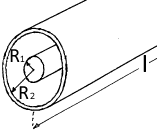
\includegraphics[width=4cm]{./pics/e-c-koaxialkabel.png}}
\parbox[t]{4.5cm}{\textbf{Doppelleitung} \\ \vspace{.2cm} \\
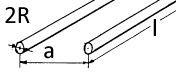
\includegraphics[width=4cm]{./pics/e-c-paralleldraht.png}}

\subsubsection{Plattenkondensator mit mehreren Dielektrika}
Grunds�tzlich kann gerechnet werden wie mit parallelen oder seriellen
Kondensatoren! Beispiel mit Luft und Dielektrika $\varepsilon_r$:
\\
\begin{tabular}{ll}
 Kapazit�t: &
$
\left.
\begin{aligned}
C_1 &= \frac{\varepsilon A}{d} = \frac{\varepsilon_0 A}{d-d_1} \\
C_2 &= \frac{\varepsilon A}{d} = \frac{\varepsilon_0 \varepsilon_r A}{d_1} 
\end{aligned}
\right\}
\quad C= \frac{C_1C_2}{C_1+C_2}
$ \\
\end{tabular}
\parbox{6.5cm}{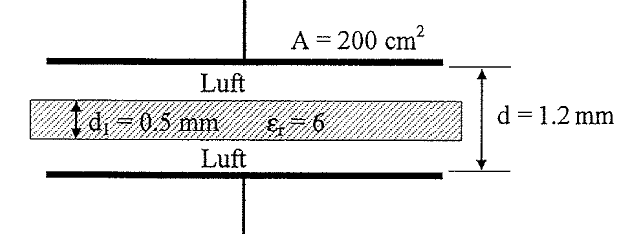
\includegraphics[width=6cm]{./pics/kond2dielekt.png}} \\

  
\subsection{Polarisation und Dielektrika}
\begin{tabular}{ll}
Im Homogenen Feld:&
$\frac{E_1}{E_2}=\frac{\epsilon_2}{\epsilon_1} $\\
Plattenkondensatoren mit verschiedenen Dielektrizit�tskonstanten: &
$U = E_1 d_1 + E_2 d_2 = \frac{D}{\epsilon_1} d_1 + \frac{D}{\epsilon_2} d_2
\Rightarrow D = \frac{U}{\frac{d_1}{\epsilon_1} + \frac{d_2}{\epsilon_2}}
\Rightarrow E_1 = \frac{D}{\epsilon_1}$\\
\end{tabular}

\parbox[t]{8.7cm} {
  \subsubsection{Feldlinien an Grenzfl. versch. Dielektrika}
  \parbox{4.5cm}{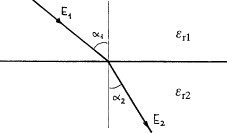
\includegraphics[width=4cm]{./pics/e-grenzflaechen-dielektrika}}
  \parbox{3.5cm}{
  $$ \frac{\tan(\alpha_1)}{\tan(\alpha_2)} = \frac{\varepsilon_{r1}}{\varepsilon_{r2}} $$ }
}
\parbox[t]{9.4cm}{
\subsubsection{Eigenschaften von Dielektrika}
  \tabcolsep0pt
  \begin{tabular}[t]{p{5.2cm} p{4.8cm}}
    homogen: $\varepsilon_r$ ist ortsunabh�ngig 
      & inhomogen: $\varepsilon_r$ ist ortsabh�ngig \\
    linear: $\varepsilon_r$ ist feldst�rkeunabh. 
      & nichtlinear: $\varepsilon_r$ ist feldst�rkeabh. \\ 
    isotrop: $\varepsilon_r$ ist richtungsunabh. 
      & anisotrop: $\varepsilon_r$ ist richtungsabh. 
  \end{tabular}
}

\subsection{Energie und Kraft im elektrostatischen Feld}
Im Kondensator gespeicherte Energie: $\qquad W = \frac{1}{2} \cdot C \cdot U^2 = \frac{1}{2} \cdot Q \cdot U = \frac{1}{2} \cdot \frac{Q^2}{C}$ \\
\parbox{5cm}{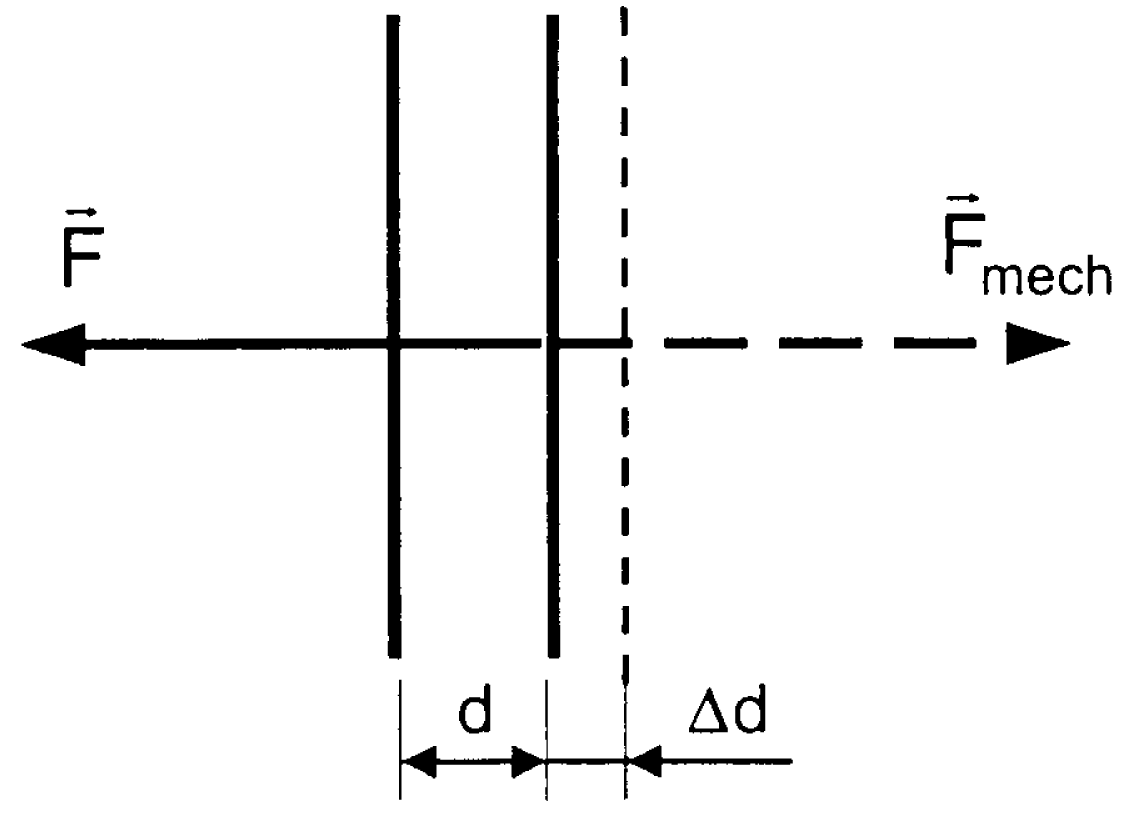
\includegraphics[width=4cm]{./pics/e-c-kraft}}
\parbox{13cm}{
  Grunds�tzlich versuchen sich die Feldlinien zu verk�rzen $\rightarrow$ Die Kraft auf die Grenzfl�chen ist so gerichtet, dass sie die Kapazit�t zu vergr�ssern sucht. \\ 
  Die Kraft berechnet sich mittels dem \textbf{Prinzip der virtuellen Verschiebung}. \\ \\
  $\qquad F = F_{mech} = \left| \frac{\Delta W}{\Delta d} \right| \qquad$ 
  $\Delta W = \frac{1}{2} \varepsilon \cdot E^2 \cdot A \cdot \Delta d \quad
  \Rightarrow \quad F = \frac{1}{2} \varepsilon \cdot E^2 \cdot A = \frac{1}{2}
  \varepsilon \cdot \frac{U^2}{d^2} \cdot A$ \\ $$ F =
  \frac{1}{2} \cdot U^2 \cdot \frac{\Delta C}{\Delta d}, \text{ (f�r U = const.)} \qquad \text{ oder } \qquad F = \frac{1}{2} \cdot Q^2 \cdot
  \frac{\mathrm d}{\Delta d} \left( \frac{1}{C} \right), \text{ (f�r Q =
  const.)}$$ \\
  Die Formel $F = \frac{1}{2}\varepsilon \cdot E^2 \cdot A$ gilt auch f�r
  Kondensatoren mit mehreren Dielektrika. Dazu wird einfach ein bekanntes
  $\varepsilon$ mit dem zugeh�rigen $E$ verwendet.}
  
  
\subsection{Das elektrische Feld meherer Punktladungen}
\begin{multicols}{2}
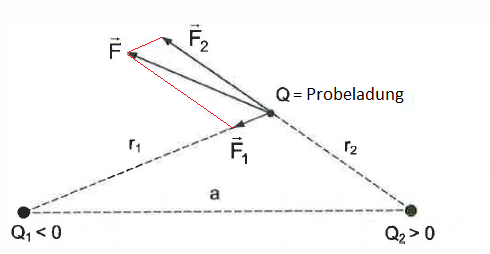
\includegraphics[width=6cm]{./pics/f_2pkt_probeladung.png} 
$\vec{F}=\vec{F_1}+\vec{F_1} = Q \cdot E_1 + Q \cdot E_2$\\
$\vec{E}= \vec{E_1} + \vec{E_2}$\\
$\vec{E}= \vec{E_1} + \vec{E_2} + \ldots + \vec{E_n} =
\sum\limits_{n}^{i=1}\vec{E_i}=\sum\limits_{n}^{i=1}\frac{Q_i}{4\pi\epsilon
{r_i}^2}\vec{e}_{ri} $\\
\end{multicols}
\section{Das Magnetische Feld}

\subsection{Energie und Kraft im magnetischen Feld}
\textbf{Energiedichte:}
$\boxed{w_m=\int_0^B{\vec{H}\cdot d\vec{B}}}$ (Allgemein)
$\qquad\boxed{w_m=\frac{1}{2}B\cdot H}$ (homog. Feld) $\qquad [w_m]=\frac{J}{m^3}$\\

\textbf{Energie:}
$\boxed{W_m = \frac{1}{2} \cdot L \cdot I^2=\frac{1}{2}\cdot N \cdot I \cdot
\Phi \; \text{ or } \; W_m=\frac{1}{2} \int_V \vec H \cdot
\vec B \cdot dV}$ (Allg.)
$\quad\boxed{W_m=w_m \cdot V=\frac{1}{2} \cdot B \cdot H \cdot V}$ (homog. Feld)\\
%\parbox{5cm}{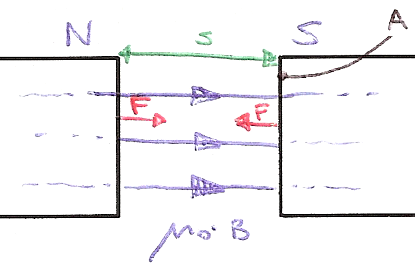
\includegraphics[width=4cm]{./pics/m-kraft-mfeld.png}}
\parbox{13cm}{	
	Die Kraft auf Grenzfl�chen ist stets so gerichtet, dass sie die Induktivit�t
	zu vergr�ssern sucht. Das heisst immer vom ferromagnetischen Material zur
	nichtferromagnetischen Umgebung (z.B. Luft). Prinzip der virtuellen
	Verschiebung:\\
	$$\boxed{F = \left| \frac{\mathrm dW_m}{\mathrm ds} \right| = \frac{1}{2} I^2 \cdot \frac{\mathrm dL}{\mathrm ds} 
	\qquad oder \qquad  F = \frac{1}{2} \cdot B \cdot H \cdot A=\frac{1}{2} \cdot
	\frac{B^2}{\mu} \cdot A \text{ (f�r } \mu_{rFe} \gg  \text{ 1)}}$$ }


\subsection{Wichtigste Formeln}

Magnetische Feldlinien verlaufen ausserhalb eines Magneten vom Nord- zum S�dpol
und sind immer geschlossen.\\ 
	\begin{tabular}[c]{ | p{5cm} | p{8cm} | p{4cm} | }
		\hline
		\textbf{Name} & \textbf{Formel} & \textbf{Einheit}\\
		\hline
		Permeabilit�tskonstante & $\mu_0 = 4 \pi \cdot 10^{-7}$ & $\frac{Vs}{Am}$\\
		\hline
		Permeabilit�t
		& $\mu = \mu_0 \mu_r = \mu_r 4 \cdot \pi \cdot 10^{-7} \frac{Vs}{Am} = \mu_r 1.2566 \frac{\mu H}{m}=\frac{B}{H}$
		&$\frac{\mu H}{m}=\frac{Vs}{An}$\\
		& $\mu_{eff}=\frac{B}{\mu_0 H_{eff}} =
		\frac{\mu_r}{1+\mu_0\frac{l_{Luft}}{l_{FE}}}$ &\\ \hline
		Magn. Flussdichte %B = \frac{\mu}{4 \pi} \cdot \frac{Q v}{r^2} =
		& $B = \frac{F}{Q \cdot v} = H \mu \text{, wobei } \vec{v} \perp
		\vec{B}$ & $\frac{Vs}{m^2} = T$ (Tesla) \\
		\hline
		Lorentzkraft
		& $\vec{F} = Q (\vec{v} \times \vec{B})=I(\vec{l}\times \vec{B}) \hspace{1cm} |\vec{F}| = Q \cdot v \cdot B
		\cdot \sin\alpha$
		&$N$\\
		Amp�resches Gesetz
		&$F=\frac{Q_2\cdot v_2 \cdot Q_1 \cdot v_1 \cdot \mu}{r^2 \cdot 4\pi}$
		&\\
		\hline
		\textbf{3-Finger-Regel: (rechte Hand)}
		& $F$ = Daumen, $v$ = Zeigefinger, $B$ = Mittelfinger
		& Bei $Q < 0$ wechselt Richtung von B!\\
		\hline
		Magnetische Feldst�rke
		& $\vec{H} = \frac{ \vec{B}}{\mu }$
		& $\frac{A}{m}$\\
		Biot-Savart
		&$H$ (bei Punkt P) $= \frac{I}{4\pi} \int \frac{\vec{dl} \times
		\vec{r(l)}}{r^3(l)}$&\\
		& $H_{eff}= \frac{\Theta_{Ges}}{l_{FE}}$ & \\ \hline
		Magnetische Spannung
		& $V_{mAB} = \int\limits \vec{H}(s) \cdot \vec{ds}$ ($V_m$ ist abh�ngig vom
		Weg) & $A$ \\
		\hline
		Durchflutung
		& $\Theta = \oint\vec{H} \cdot \vec{ds} = \int\limits \vec{J}
		\cdot \vec{dA} \vee \underbrace{\sum I_k}_{= N I} = V_m$
		& $A$\\
		\hline
		Magnetischer Fluss
		& $\Phi = \int \vec{B} \vec{dA}$
		& $Vs = Wb$ (Weber)\\
		& $\Phi = B \cdot A \cdot \cos(\gamma)$
		& B homogen\\
		\hline
		\textbf{Maxwell-Gesetz}
		& $\oint \vec{B} \vec{dA} = 0$ (vgl. Kirchhoff 1 ($\sum I = 0$))
		&\\
		\hline
		F�llfaktor
		&$F=\frac{A_{Effektiv Fe}}{A_{Tot}}$
		& $[-]$\\
		\hline
		Magn. Widerstand
		& $R_m = \frac{V_m}{\Phi} = \frac{\Theta}{\Phi} = \frac{l}{\mu A} $
		& $\frac{A}{Wb}$ \\
		``Ohmsches	Gesetz des Magn.``
		&&\\
		\hline
		Magn. Leitwert
		& $\Lambda = \frac{1}{R_m} = \frac{\Phi}{V_m}=\frac{\Phi}{\Theta}$
		& $\frac{Vs}{A} = H$ (Henry) (Im Formelbuch als $A_L$)\\
		\hline
		Verketteter Fluss
		& $\Psi = \sum \Phi $ (meist $\Psi = N \Phi$)
		& $[\Psi] = [\Phi] = Vs = Wb$\\
		\hline
		Induktivit�t
		& $L = \frac{\Psi}{I}  \qquad \text{Bei idealer Koppl.: } L = \Lambda N^2 = \frac{N^2}{R_m} $
		& $[L] = \frac{Vs}{A} = H$\\
		\hline
		Gegeninduktivit�t
		& $M = M_{21} = M_{12}$ Bei idealer Koppl. $M = \sqrt{L_1 L_2}$
		& vorder Index = Wirkung,\\
		&$M_{21} = \frac{\Psi_{21}}{I_1}$  (meist $M_{21} = \frac{N_2 \Phi_{21}}{I_1}$)
		& hinterer = Ursache\\
		\hline
		Kopplungsfaktor
		& $k = \frac{M}{\sqrt{L_1 L_2}}$ Bei idealer Kopplung: $k = 1$
		& $[-]$ \\
		\hline
		Streukoeffizient
		& $\sigma = 1 - k^2 = 1 -\frac{M^2}{L_1 L_2}$ Bei idealer Kopplung: $\sigma = 0$
		& $[-]$\\
		\hline
		Kreis-r in M-Feld abgelenkte Q
		& $ m_e = 9,11 \cdot 10^{-31} kg$
		& $r = \frac{m_Q \cdot v}{Q \cdot B}$ \\
		\hline
	\end{tabular}
	
\subsection{Diverse Formeln bzgl. Magnetismus}
\begin{tabular}[c]{l l}
$\text{Hall-Sonde: }$
&$\text{Kraft auf stromf�hrende Leiter: }$\\ 
$U_H = \frac{I \cdot B}{e \cdot n_p \cdot h}$
&$\vec{F_L} = I (\vec{l} \times \vec{B}) \qquad F_L = I \cdot l \cdot B \cdot \sin{\alpha}$\\

Magnetfeld ausserhalb eines langen Leiters:
&Magnetfeld innerhalb eines geraden, langen Leiters: \\
$H(r) = \frac{I}{2 \cdot \pi \cdot r}$
&$H(r) = \frac{I}{2 \pi r} \frac{A_{eingeschlossen}}{A_{total}} = 
 \frac{I}{2 \pi} \frac{r}{r_a^2}$\\
Magnetfeld der Zylinderspule:
&Magnetfeld einer Toroidspule:\\
$H(r) = \frac{N \cdot I}{l}= \frac{\theta}{l} \qquad l \gg d$
& $H_{innen}(r) = \frac{N \cdot I}{2 \cdot \pi \cdot r \to l} \qquad H_{aussen}
= 0$
\end{tabular}

Siehe \ref{seich}

\subsection{Zusammenstellung magnetischer Gr�ssen f�r spezielle
Leiteranordnungen}
\begin{tabular}{|p{5cm}|l|l|l|l|l|}
  \hline
  & Leitwert $ \Lambda $ & Durchfl. $ \Theta $ & Fluss $ \Phi ^{1)} $ &
  Verk.-Fluss $ \Psi $ & Induktivit�t $L^{2)}$ \\
  \hline
  Kreisf�rmige Schleife & $\frac{\mu D}{2}\cdot\ln\frac{D}{d}$ & $\Theta = I$ & $\frac{\mu D}{2}\cdot\ln\frac{D}{d}\cdot I$ & $\Psi = \Phi$ & $L=\frac{\mu
  D}{2}\cdot\ln\frac{D}{d}$\\
  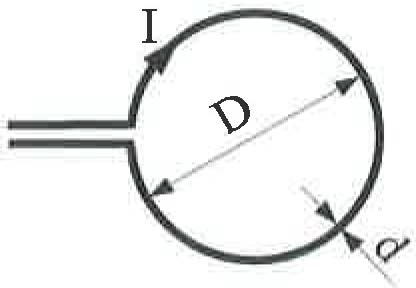
\includegraphics[width=3cm]{./pics/kreisfoermige_schleife.png} & & & & & \\
  \hline
  Kreisrahmenspule$^{3)}$ & $\frac{\mu D}{2}\cdot\ln\frac{D}{d}$ & $\Theta = NI$ & $\frac{\mu D}{2}\cdot\ln\frac{D}{d}\cdot N \cdot I$ & $\Psi = N \cdot \Phi$ & $L=\frac{\mu  D}{2}\cdot\ln\frac{D}{d}\cdot N^2$\\
  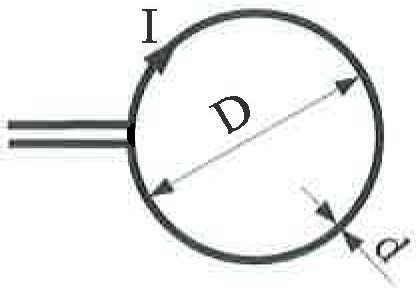
\includegraphics[width=3cm]{./pics/kreisrahmenspule.png} & & & & & \\
  \hline
  Zylinderspule $l \gg d$
  & $\frac{\mu A}{l} = \frac{\mu \pi d^2}{4l}$ & $\Theta = NI$ & $\frac{\mu \pi d^2}{4l} \cdot N \cdot I$ & $\Psi = N \cdot \Phi$ & $L=\frac{\mu \pi d^2}{4l}\cdot N^2$\\
  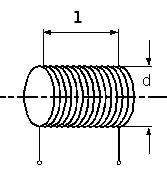
\includegraphics[width=3cm]{./pics/zylinderspule.png} & & & & & \\
  \hline
  Toroidspule $^{4)}$ & $\frac{\mu A}{l_m} = \frac{\mu d^2}{4 D_m}$ & $\Theta = NI$ & $\frac{\mu d^2}{4 D_m}\cdot N \cdot I$ & $\Psi = N
  \cdot \Phi$ & $L=\frac{\mu d^2}{4 D_m}\cdot
  N^2$\\
  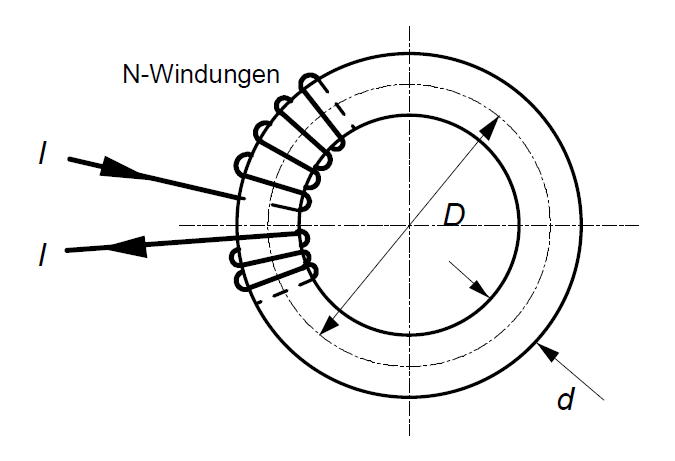
\includegraphics[width=4cm]{./pics/toroidspule.png} & & & & & \\
  \hline
  Ringspule mit rechteckf. Querschnitt & $\frac{\mu a}{2
  \pi}\cdot\ln\frac{D}{d}$ & $\Theta = NI$ & $\frac{\mu a}{2\pi}\cdot\ln\frac{D}{d}\cdot N \cdot I$ & $\Psi = N
  \cdot \Phi$ & $L=\frac{\mu a}{2\pi}\cdot\ln\frac{D}{d}\cdot N^2$\\
  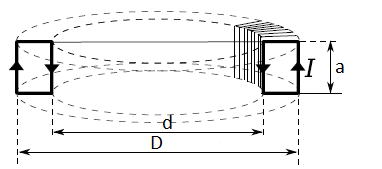
\includegraphics[width=5cm]{./pics/torus.png} & & & & & \\
  \hline
  Koaxialleitung $R_2 > R_1$
  & $\frac{\mu l}{2 \pi}\cdot\ln\frac{R_2}{R_1}$ & $\Theta = I$ & $\frac{\mu l}{2\pi}\cdot\ln\frac{R_2}{R_1}\cdot I$ & $\Psi = \Phi$ & $L=\frac{\mu l}{2\pi}\cdot\ln\frac{R_2}{R_1}$ \\
  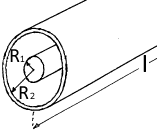
\includegraphics[width=3cm]{./pics/e-c-koaxialkabel.png} & & & & & \\
  \hline
  Paralleldrahtleitung $l \gg a \gg R$ & $\frac{\mu l}{\pi}\cdot\ln\frac{a-R}{R}$ & $\Theta = I$ & $\frac{\mu l}{\pi}\cdot\ln\frac{a-R}{R}\cdot I$ & $\Psi = \Phi$ & $L=\frac{\mu l}{\pi}\cdot\ln\frac{a-R}{R}$\\
  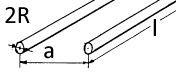
\includegraphics[width=3cm]{./pics/e-c-paralleldraht.png} & & & & & \\
  \hline
\end{tabular}

\begin{tabular}{p{8.5cm}p{8.5cm}}
  \textbf{Bemerkungen:} & \textbf{Allgemein:} \\
  $1) $ ohne Fluss durch Leiter & $\Phi = \Lambda \cdot \Theta , \Lambda =
  \frac{1}{R_m}$\\
  $2) $ nur �ussere Induktivit�t & $L=\frac{\Psi}{I}$\\
  $3) A=\frac{\pi d^2}{4}\ \ l_m \approx \pi D_m$ & $L=\Lambda=\frac{1}{R_m},
  falls N=1$ \\
  $4) $ Wickeldurchmesser d in radialer und axialer Richtung $d\ll D$ &
  $L=\Lambda N^2 =\frac{N^2}{R_m}$, falls die N-Windungen unter sich ideal
  gekoppelt sind.
\end{tabular}

%%%%%%%%%%
%%EDIT!!!
%%%%%%%%%%

\subsection{Der magnetische Kreis}

\subsubsection{Ohne Luftspalt}
  \begin{tabular}{|l|l|}
    \hline
    Magnetische Spannung & $V_m=\Theta=H_{Fe}\cdot l_{Fe}$\\
    \hline
    ``Ohmsches'' Gesetz, Polfluss & $\Phi = \frac{V_m}{R_m}$\\
    \hline
    Reluktanz & $R_m=\frac{l_{Fe}}{\mu_{Fe}\cdot A_{Fe}}$\\
    \hline
    Permeanz & $\Lambda_m = \frac{1}{R_m}$\\
    \hline
  \end{tabular}
  
\subsubsection{Mit Luftspalt}
  \begin{tabular}{|l|l|l|l|}
    \hline
    & Eisen & Luftspalt & Permanentmagnet \\
    \hline
    Widerstand & $R_{Fe}=\frac{l_{Fe}}{\mu_{Fe}\mu_0A_{Fe}}$ & $R_L =
    \frac{l_{L}}{\mu_0\cdot A_L}$ & \\
    \hline
    Fluss $\Phi$ & $ \Phi_{Fe}=B_{Fe} \cdot
    A_{Fe}$ & $ \Phi_{L}=B_{L}A_{L}$ & $B_{M}\cdot A_{M}$ \\
    \hline
    Flussdichte & $ B_{Fe}=\mu_0\mu_{Fe}H_{Fe}$ & $B_L=\mu_0H_L$ &
    $B_M=\mu_0\mu_MH_M+M$\\
    \hline
    magnetische Teilspannung & $V_{mFe}=l_{Fe}\cdot H_{Fe}$ & $V_L = L\cdot H_L$
    & $V_{M} = l_MH_M$ \\
    \hline 
  \end{tabular}
  $\text{Magnetische Spannung } = \Theta = V_m = V_{Fe}+V_L+V_M = N\cdot I \cong
  l_M\frac{B_M-M}{\mu_0\mu_M}+lH_L$ \\
  Eine Streuung mit Faktor $0\le\sigma\le 1$ kann als
  Widerstand parallel zu $R_L$ angesehen werden: \\
  $R=\frac{R_{\sigma}\cdot R_{\delta}}{R_{\sigma}+R_{\delta}}$\\
  Streufluss $\Phi_{\sigma} \approx 5\%\Phi_L $\\
  Streufaktor $\sigma = \frac{\Phi_{\sigma}}{\Phi}$\\
  Der Fluss im Luftspalt $\Phi_L $ �ndert dann zu $
  \Phi_{L}=(1-\sigma)B_{L}A_{L} $ \\
  
\subsubsection{Arbeitspunkt AP}
$H^*=\frac{H^*}{1+\frac{l_M}{l_L}\frac{\mu_0H^*}{B^*}}$\\
$B^*=\frac{\mu_0H^*}{\frac{l_L}{l_M}+\frac{\mu_0H^*}{B^*}}$\\
$B_{opt}=\frac{1}{2}B^*, H_{opt}=-\frac{1}{2}H^*$\\
$l_M=\mu_Ml_L$

\subsubsection{Von der Durchflutung $\Theta$ ausgehende Berechnung}
\begin{minipage}{11cm}
  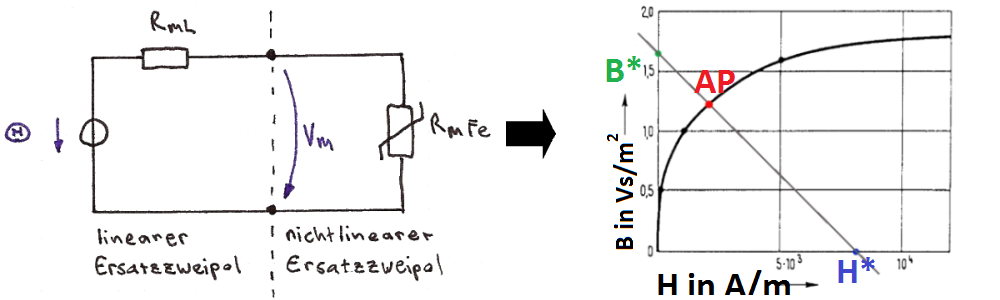
\includegraphics[width=11cm]{./pics/magnetischerkreis2.png}
\end{minipage}
\hfill
\begin{minipage}{7cm}
\begin{tabbing}
xxx \= \kill  
1. \> magn. Kreis in linearen und nichtlinearen\\
   \> Teil aufteilen\\
2. \> Leerlaufspannung $V_{mLeerlauf}$ und\\
   \> Kurzschlussfluss $\Phi_k$ bestimmen\\
3. \> $H^*$ und $B^*$ bestimmen\\
4. \> $H^*$ und $B^*$ einzeichnen und\\
   \> Arbeitspunkt $AP$ bestimmen\\
5. \> $H$ und $B$ im AP herauslesen
\end{tabbing}
\end{minipage}
$$V_{mLeerlauf}=\Theta \qquad \Phi_k=\frac{\Theta}{R_{mL}}=\frac{\Theta \cdot
\mu_0 \cdot A_L }{l_L} \qquad H^*=\frac{\Theta}{l_{Fe}} \qquad B^*=\frac{\Phi_k}{A_{Fe}}=\frac{\Theta \cdot
\mu_0 \cdot A_L }{l_L A_{Fe}}=\overbrace{\frac{\mu_0 \cdot
\Theta}{l_L}}^{A_L=A_{Fe}}$$ 
\subsection{Kraft im Magnetfled}
$\vec{B} = \mu_0 \cdot \vec{H}$ homogen, $l=$ Leiterl"ange, $y=$ Abstand zum
Leiter\\
\begin{multicols}{3}
	\subsubsection{Stromkraft I (Motorprinzip)} 
	
	\begin{itemize}
		\setlength{\itemsep}{1pt}
		\setlength{\parskip}{0pt}
		\setlength{\parsep}{0pt}
		
		\item $F=B \cdot I \cdot l \Leftrightarrow \frac{F}{l}= B \cdot I$\\
		\item $\vec{F} = -\vec{e} y I \cdot B \cdot l = -\vec{e}yF $
	\end{itemize}
	\subsubsection{Stromkraft II (Generatorprinzip)}
		\begin{itemize}
		\setlength{\itemsep}{1pt}
		\setlength{\parskip}{0pt}
		\setlength{\parsep}{0pt}
		
		\item  $U_{ind} = B \cdot l \cdot v$
	\end{itemize}

	\subsubsection{Reluktanzkraft}
	\begin{itemize}
		\setlength{\itemsep}{1pt}
		\setlength{\parskip}{0pt}
		\setlength{\parsep}{0pt}
		
		\item $F_{l_L} = \frac{B^2 \cdot A}{2\cdot \mu_0} $
		\item Motorendrehmoment \\ $M = \frac{\mu_0 (I \cdot N)^2 \cdot r \cdot
		l_Fe}{4 l_L}$
	\end{itemize}
\end{multicols}		

\subsubsection{Ferromagnetische Stoffe}
Siehe \ref{ferromagnetische_stoffe}

\begin{landscape}
\section{Anhang}
\subsection{Diverse Formeln bzgl. Magnetismus} \label{seich}
\begin{tabular}{llll}
  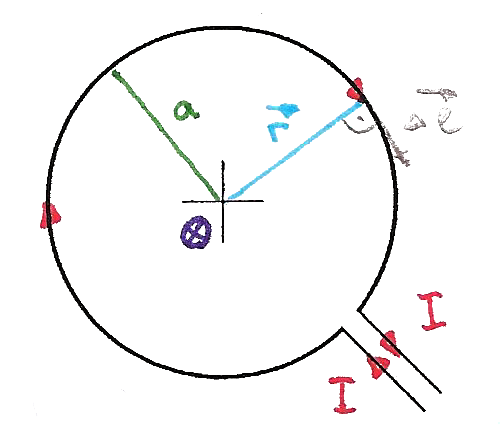
\includegraphics[width=5.7cm]{./pics/biot1.png} &
  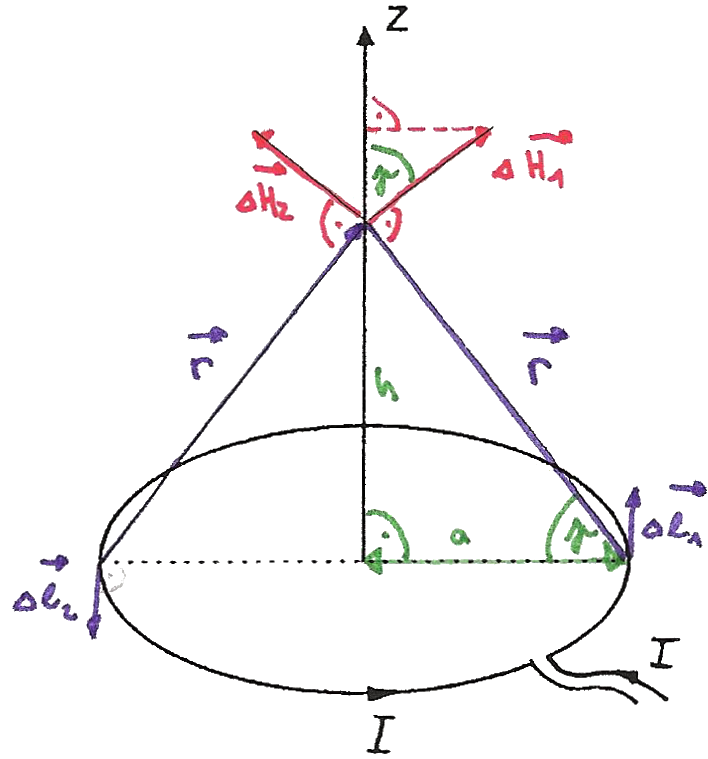
\includegraphics[width=5.7cm]{./pics/biot2.png} &
  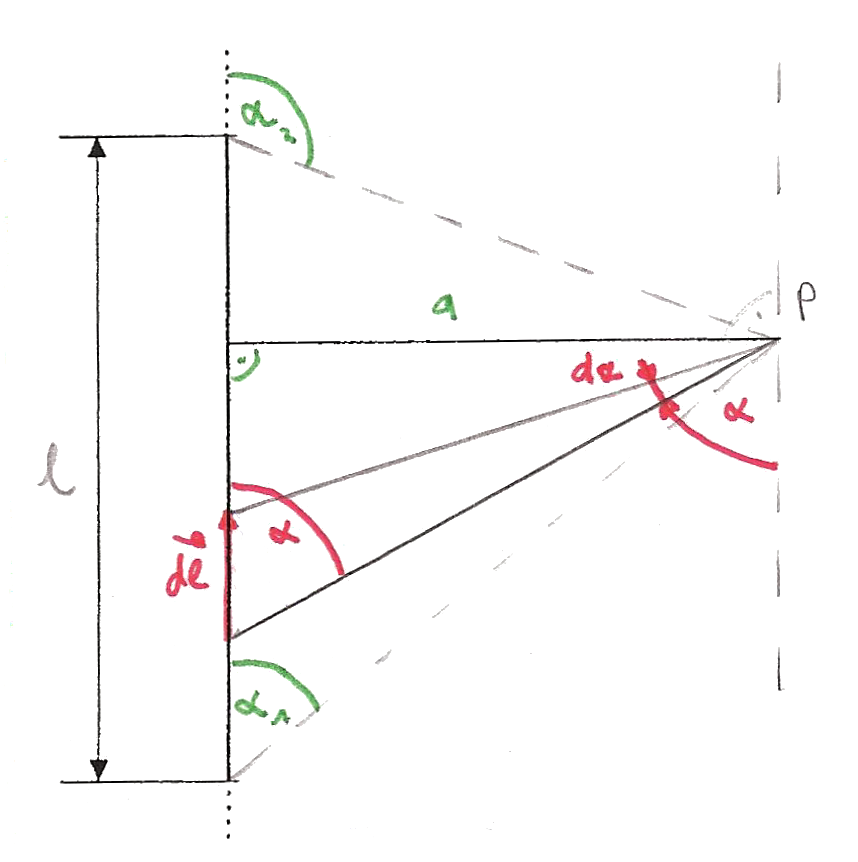
\includegraphics[width=5cm]{./pics/biot3.png} &
  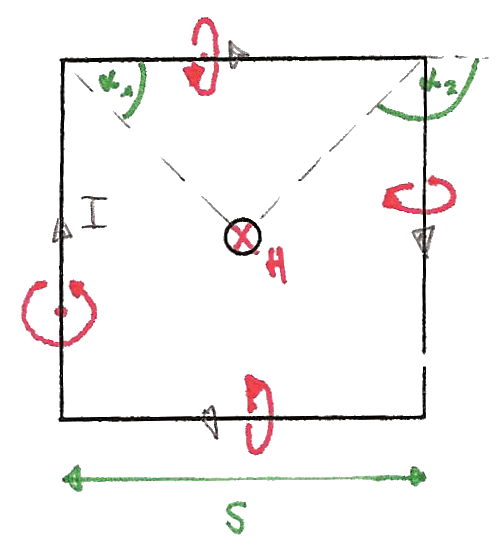
\includegraphics[width=5.7cm]{./pics/biot4.png} \\
  $H =\frac{I}{D} = \frac{I}{2a}$ &
  $H=\frac{I}{2} \cdot \frac{a^2}{\sqrt{a^2+h^2}^3}$ &
  $H=\frac{I}{4\pi a}(\cos(\alpha_1)- \cos(\alpha_2))$ &
  $H= \frac{I \cdot 2 \sqrt{2}}{\pi \cdot s}$ \\
\end{tabular}

\subsection{Ferromagnetische Stoffe} \label{ferromagnetische_stoffe}
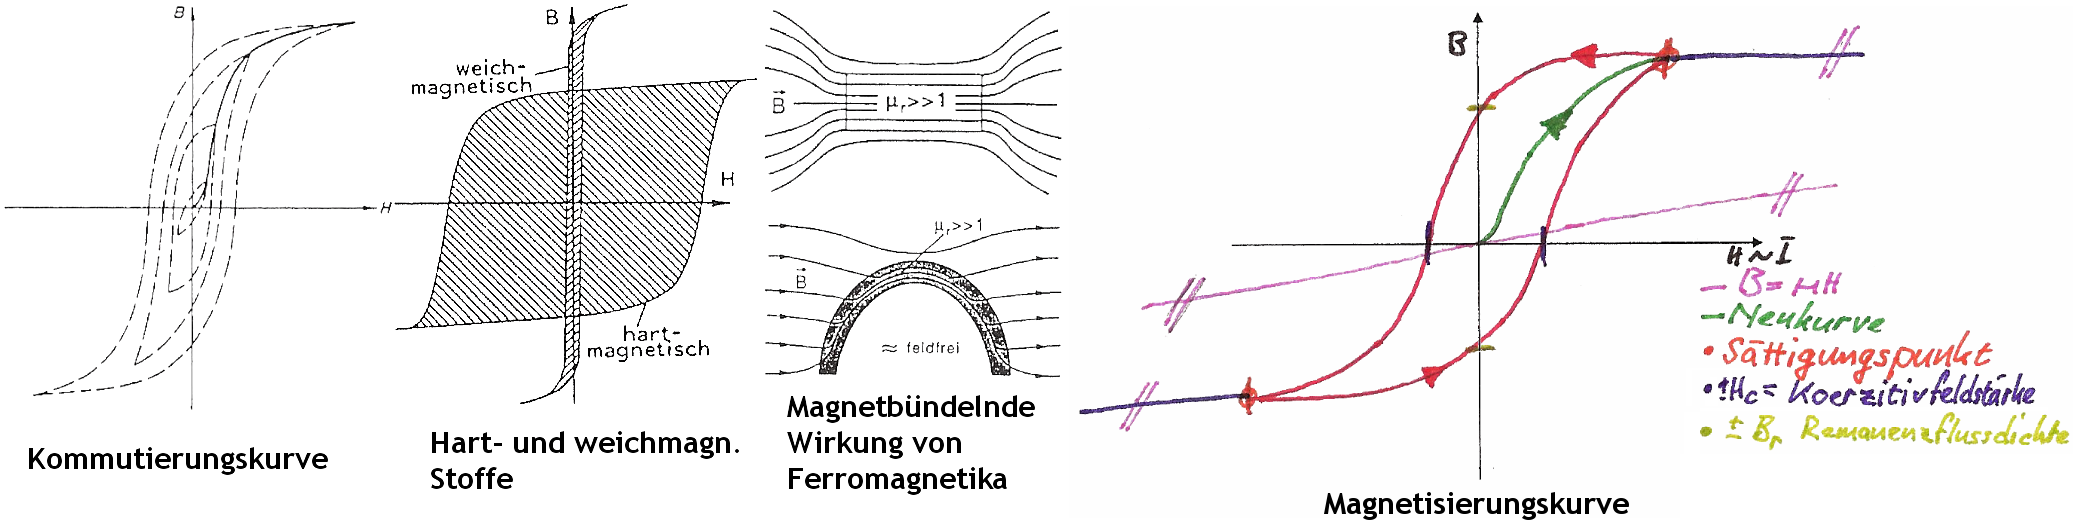
\includegraphics[width=25cm]{./pics/magnetisierung.png}


\end{landscape}
\section{Idiotenseite}
\subsection{SI Vors�tze}
  \begin{tabular}{|l|l|l||l|l|l|}
    \hline
    Dezi & d & $10^{-1}$ 		& Deka & da & $10^{1}$ \\
    \hline
    Zenti & c & $10^{-2}$ 		& Hekto & h & $10^{2}$ \\
    \hline
    Milli & m & $10^{-3}$ 		& Kilo & k & $10^{3}$ \\
    \hline
    Mikro & $\mu$ & $10^{-6}$ 	& Mega & M & $10^{6}$ \\
    \hline
    Nano & n & $10^{-9}$ 		& Giga & G & $10^{9}$ \\
    \hline
    Piko & p & $10^{-12}$		& Tera & T & $10^{12}$ \\
    \hline
    Femto & f & $10^{-15}$ 		& Peta & P & $10^{15}$ \\
    \hline
  \end{tabular}
\subsection{Fl�chenumrechnungen}
  $1dm^2 = 10^{-2}m^2$ \\
  $1cm^2 = 10^{-4}m^2$ \\
  $1mm^2 = 10^{-6}m^2$ \\
  $1\mu m^2 = 10^{-12}m^2$\\
\subsection{Volumenumrechnungen}
  $1dm^3 = 10^{-3}m^3$ \\
  $1cm^3 = 10^{-6}m^3$ \\
  $1mm^3 = 10^{-9}m^3$ \\
\subsection{Dreieck}
  \begin{tabular}{ll}
    Umkreisradius & $r=\frac{a}{2\sin{\alpha}}$\\
  \end{tabular}
\subsection{Kreis}
  \begin{tabular}{ll}
    Fl�che & $A=r^2\pi$ \\
    Kreisringfl�che & $A=\pi (r_a^2-r_i^2$\\
    Umfang & $u=2r\pi$ \\
  \end{tabular}
\subsection{Kugel}
  \begin{tabular}{ll}
    Volumen & $V=\frac{4}{3}\pi r^3$\\
    Oberfl�che & $A=4\pi r^2$\\
  \end{tabular}

\end{document}

